\chapter{Dynamic programming}

\index{dynamic programming}

\key{Dynamic programming}
is a technique that combines the correctness
of complete search and the efficiency
of greedy algorithms.
Dynamic programming can be applied if the
problem can be divided into overlapping subproblems
that can be solved independently.

There are two uses for dynamic programming:

\begin{itemize}
\item
\key{Finding an optimal solution}:
We want to find a solution that is
as large as possible or as small as possible.
\item
\key{Counting the number of solutions}:
We want to calculate the total number of
possible solutions.
\end{itemize}

We will first see how dynamic programming can
be used to find an optimal solution,
and then we will use the same idea for
counting the solutions.

Understanding dynamic programming is a milestone
in every competitive programmer's career.
While the basic idea of the technique is simple,
the challenge is how to apply it to different problems.
This chapter introduces a set of classic problems
that are a good starting point.

\section{Coin problem}

We first discuss a problem that we
have already seen in Chapter 6:
Given a set of coin values $\{c_1,c_2,\ldots,c_k\}$
and a sum of money $x$, our task is to
form the sum $x$ using as few coins as possible.

In Chapter 6, we solved the problem using a
greedy algorithm that always selects the largest
possible coin.
The greedy algorithm works, for example,
when the coins are the euro coins,
but in the general case the greedy algorithm
does not necessarily produce an optimal solution.

Now it is time to solve the problem efficiently
using dynamic programming, so that the algorithm
works for any coin set.
The dynamic programming
algorithm is based on a recursive function
that goes through all possibilities how to
form the sum, like a brute force algorithm.
However, the dynamic programming
algorithm is efficient because
it uses \emph{memoization} and
calculates the answer to each subproblem only once.

\subsubsection{Recursive formulation}

The idea in dynamic programming is to
formulate the problem recursively so
that the answer to the problem can be
calculated from answers to smaller
subproblems.
In the coin problem, a natural recursive
problem is as follows:
what is the smallest number of coins
required for constructing a sum $x$?

Let $f(x)$ be a function that gives the answer
to the problem, i.e., $f(x)$ is the smallest
number of coins required for constructing a sum $x$.
The values of the function depend on the
values of the coins.
For example, if the coin values are $\{1,3,4\}$,
the first values of the function are as follows:

\[
\begin{array}{lcl}
f(0) & = & 0 \\
f(1) & = & 1 \\
f(2) & = & 2 \\
f(3) & = & 1 \\
f(4) & = & 1 \\
f(5) & = & 2 \\
f(6) & = & 2 \\
f(7) & = & 2 \\
f(8) & = & 2 \\
f(9) & = & 3 \\
f(10) & = & 3 \\
\end{array}
\]

First, $f(0)=0$ because no coins are needed
for the sum $0$.
Moreover, $f(3)=1$ because the sum $3$
can be formed using coin 3,
and $f(5)=2$ because the sum 5 can
be formed using coins 1 and 4.

The essential property in the function is
that each value of $f(x)$ can be calculated
recursively from smaller values of the function.
For example, if the coin set is $\{1,3,4\}$,
there are three ways to select the first coin
in a solution: we can choose coin 1, 3 or 4.
If coin 1 is chosen, the remaining task is to
form the sum $x-1$.
Similarly, if coin 3 or 4 is chosen,
we should form the sum $x-3$ or $x-4$.

Thus, the recursive formula is
\[f(x) = \min(f(x-1),f(x-3),f(x-4))+1\]
where the function $\min$ gives the smallest
of its parameters.
In the general case, for the coin set
$\{c_1,c_2,\ldots,c_k\}$,
the recursive formula is
\[f(x) = \min(f(x-c_1),f(x-c_2),\ldots,f(x-c_k))+1.\]
The base case for the function is
\[f(0)=0,\]
because no coins are needed for constructing
the sum 0.
In addition, it is convenient to define
\[f(x)=\infty\hspace{8px}\textrm{if $x<0$}.\]
This means that an infinite number of coins
is needed for forming a negative sum of money.
This prevents the function from constructing
a solution where the initial sum of money is negative.

Once a recursive function that solves the problem
has been found,
we can directly implement a solution in C++:

\begin{lstlisting}
int f(int x) {
    if (x < 0) return INF;
    if (x == 0) return 0;
    int u = INF;
    for (int i = 1; i <= k; i++) {
        u = min(u, f(x-c[i])+1);
    }
    return u;
}
\end{lstlisting}

The code assumes that the available coins are
stored in an array $\texttt{c}$,
and the constant \texttt{INF} denotes infinity.
This function works but it is not efficient yet,
because it goes through a large number
of ways to construct the sum.
However, the function can be made efficient by
using memoization.

\subsubsection{Memoization}

\index{memoization}

Dynamic programming allows us to calculate the
value of a recursive function efficiently
using \key{memoization}.
This means that an auxiliary array is used
for recording the values of the function
for different parameters.
For each parameter, the value of the function
is calculated recursively only once, and after this,
the value can be directly retrieved from the array.

In this problem, we can use an array
\begin{lstlisting}
int d[N];
\end{lstlisting}

where $\texttt{d}[x]$ will contain
the value of $f(x)$.
The constant $N$ has to be chosen so
that all required values of the function fit
in the array.

After this, the function can be efficiently
implemented as follows:

\begin{lstlisting}
int f(int x) {
    if (x < 0) return INF;
    if (x == 0) return 0;
    if (d[x]) return d[x];
    int u = INF;
    for (int i = 1; i <= k; i++) {
        u = min(u, f(x-c[i])+1);
    }
    d[x] = u;
    return d[x];
}
\end{lstlisting}

The function handles the base cases
$x<0$ and $x=0$ as previously.
Then the function checks if
$f(x)$ has already been stored
in $\texttt{d}[x]$.
If the value of $f(x)$ is found in the array,
the function directly returns it.
Otherwise the function calculates the value
recursively and stores it in $\texttt{d}[x]$.

Using memoization the function works
efficiently, because the answer for each parameter $x$
is calculated recursively only once.
After a value of $f(x)$ has been stored in the array,
it can be efficiently retrieved whenever the
function will be called again with the parameter $x$.

The time complexity of the resulting algorithm
is $O(xk)$ where the sum is $x$ and the number of
coins is $k$.
In practice, the algorithm can be used if
$x$ is so small that it is possible to allocate
an array for all possible function parameters.

Note that the array can also be constructed using
a loop that calculates all the values
instead of a recursive function:
\begin{lstlisting}
d[0] = 0;
for (int i = 1; i <= x; i++) {
    int u = INF;
    for (int j = 1; j <= k; j++) {
        if (i-c[j] < 0) continue;
        u = min(u, d[i-c[j]]+1);
    }
    d[i] = u;
}
\end{lstlisting}

This implementation is shorter and somewhat
more efficient than recursion,
and experienced competitive programmers
often prefer dynamic programming solutions
that are implemented using loops.
Still, the underlying idea is the same as
in the recursive function.

\subsubsection{Constructing a solution}

Sometimes we are asked both to find the value
of an optimal solution and also to give
an example how such a solution can be constructed.
In the coin problem, this means that the algorithm
should show how to select the coins that produce
the sum $x$ using as few coins as possible.

We can construct the solution by adding another
array to the code. The new array indicates for
each sum of money the first coin that should be
chosen in an optimal solution.
In the following code, the array \texttt{e}
is used for this:

\begin{lstlisting}
d[0] = 0;
for (int i = 1; i <= x; i++) {
    d[i] = INF;
    for (int j = 1; j <= k; j++) {
        if (i-c[j] < 0) continue;
        int u = d[i-c[j]]+1;
        if (u < d[i]) {
            d[i] = u;
            e[i] = c[j];
        }
    }
}
\end{lstlisting}

After this, we can print the coins needed
for the sum $x$ as follows:

\begin{lstlisting}
while (x > 0) {
    cout << e[x] << "\n";
    x -= e[x];
}
\end{lstlisting}

\subsubsection{Counting the number of solutions}

Let us now consider a variant of the problem
that is otherwise like the original problem,
but we should count the total number of solutions instead
of finding the optimal solution.
For example, if the coins are $\{1,3,4\}$ and
the target sum is $5$,
there are a total of 6 solutions:

\begin{multicols}{2}
\begin{itemize}
\item $1+1+1+1+1$
\item $1+1+3$
\item $1+3+1$
\item $3+1+1$
\item $1+4$
\item $4+1$
\end{itemize}
\end{multicols}

The number of the solutions can be calculated
using the same idea as finding the optimal solution.
The difference is that when finding the optimal solution,
we maximize or minimize something in the recursion,
but now we will calculate sums of numbers of solutions.

To solve the problem, we can define a function $f(x)$
that gives the number of ways to construct
a sum $x$ using the coins.
For example, $f(5)=6$ when the coins are $\{1,3,4\}$.
The value of $f(x)$ can be calculated recursively
using the formula
\[ f(x) = f(x-c_1)+f(x-c_2)+\cdots+f(x-c_{k}),\]
because to form the sum $x$, we have to first
choose some coin $c_i$ and then form the sum $x-c_i$.
The base cases are $f(0)=1$, because there is exactly
one way to form the sum 0 using an empty set of coins,
and $f(x)=0$, when $x<0$, because it is not possible
to form a negative sum of money.

If the coin set is $\{1,3,4\}$, the function is
\[ f(x) = f(x-1)+f(x-3)+f(x-4) \]
and the first values of the function are:
\[
\begin{array}{lcl}
f(0) & = & 1 \\
f(1) & = & 1 \\
f(2) & = & 1 \\
f(3) & = & 2 \\
f(4) & = & 4 \\
f(5) & = & 6 \\
f(6) & = & 9 \\
f(7) & = & 15 \\
f(8) & = & 25 \\
f(9) & = & 40 \\
\end{array}
\]

The following code calculates the value of $f(x)$
using dynamic programming by filling the array
\texttt{d} for parameters $0 \ldots x$:

\begin{lstlisting}
d[0] = 1;
for (int i = 1; i <= x; i++) {
    for (int j = 1; j <= k; j++) {
        if (i-c[j] < 0) continue;
        d[i] += d[i-c[j]];
    }
}
\end{lstlisting}

Often the number of solutions is so large
that it is not required to calculate the exact number
but it is enough to give the answer modulo $m$
where, for example, $m=10^9+7$.
This can be done by changing the code so that
all calculations are done modulo $m$.
In the above code, it suffices to add the line
\begin{lstlisting}
        d[i] %= m;
\end{lstlisting}
after the line
\begin{lstlisting}
        d[i] += d[i-c[j]];
\end{lstlisting}

Now we have discussed all basic
techniques related to
dynamic programming.
Since dynamic programming can be used
in many different situations,
we will now go through a set of problems
that show further examples about
possibilities of dynamic programming.

\section{Longest increasing subsequence}

\index{longest increasing subsequence}

Let us consider the following problem:
Given an array that contains $n$
numbers,
our task is to find the
\key{longest increasing subsequence}
of the array.
This is a sequence of array elements
that goes from left to right,
and each element of the sequence is larger
than the previous element.
For example, in the array

\begin{center}
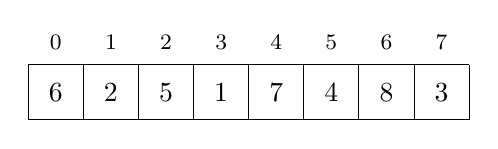
\begin{tikzpicture}[scale=0.7]
\draw (0,0) grid (8,1);
\node at (0.5,0.5) {$6$};
\node at (1.5,0.5) {$2$};
\node at (2.5,0.5) {$5$};
\node at (3.5,0.5) {$1$};
\node at (4.5,0.5) {$7$};
\node at (5.5,0.5) {$4$};
\node at (6.5,0.5) {$8$};
\node at (7.5,0.5) {$3$};

\footnotesize
\node at (0.5,1.4) {$0$};
\node at (1.5,1.4) {$1$};
\node at (2.5,1.4) {$2$};
\node at (3.5,1.4) {$3$};
\node at (4.5,1.4) {$4$};
\node at (5.5,1.4) {$5$};
\node at (6.5,1.4) {$6$};
\node at (7.5,1.4) {$7$};
\end{tikzpicture}
\end{center}
the longest increasing subsequence
contains 4 elements:
\begin{center}
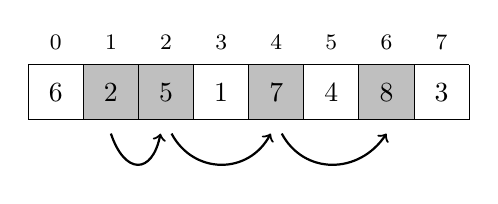
\begin{tikzpicture}[scale=0.7]
\fill[color=lightgray] (1,0) rectangle (2,1);
\fill[color=lightgray] (2,0) rectangle (3,1);
\fill[color=lightgray] (4,0) rectangle (5,1);
\fill[color=lightgray] (6,0) rectangle (7,1);
\draw (0,0) grid (8,1);
\node at (0.5,0.5) {$6$};
\node at (1.5,0.5) {$2$};
\node at (2.5,0.5) {$5$};
\node at (3.5,0.5) {$1$};
\node at (4.5,0.5) {$7$};
\node at (5.5,0.5) {$4$};
\node at (6.5,0.5) {$8$};
\node at (7.5,0.5) {$3$};

\draw[thick,->] (1.5,-0.25) .. controls (1.75,-1.00) and (2.25,-1.00) .. (2.4,-0.25);
\draw[thick,->] (2.6,-0.25) .. controls (3.0,-1.00) and (4.0,-1.00) .. (4.4,-0.25);
\draw[thick,->] (4.6,-0.25) .. controls (5.0,-1.00) and (6.0,-1.00) .. (6.5,-0.25);

\footnotesize
\node at (0.5,1.4) {$0$};
\node at (1.5,1.4) {$1$};
\node at (2.5,1.4) {$2$};
\node at (3.5,1.4) {$3$};
\node at (4.5,1.4) {$4$};
\node at (5.5,1.4) {$5$};
\node at (6.5,1.4) {$6$};
\node at (7.5,1.4) {$7$};
\end{tikzpicture}
\end{center}

Let $f(k)$ be the length of the
longest increasing subsequence
that ends at position $k$.
Using this function, the answer to the problem
is the largest of the values
$f(0),f(1),\ldots,f(n-1)$.
For example, in the above array
the values of the function are as follows:
\[
\begin{array}{lcl}
f(0) & = & 1 \\
f(1) & = & 1 \\
f(2) & = & 2 \\
f(3) & = & 1 \\
f(4) & = & 3 \\
f(5) & = & 2 \\
f(6) & = & 4 \\
f(7) & = & 2 \\
\end{array}
\]

When calculating the value of $f(k)$,
there are two possibilities how the subsequence
that ends at position $k$ is constructed:
\begin{enumerate}
\item The subsequence
only contains the element at position $k$. In this case $f(k)=1$.
\item The subsequence contains a subsequence
that ends at position $i$ where $i<k$,
followed by the element at position $k$.
The element at position $i$ must be smaller
than the element at position $k$.
In this case $f(k)=f(i)+1$.
\end{enumerate}

For example, in the above example $f(6)=4$,
because the subsequence $[2,5,7]$ of length 3
ends at position 4, and by adding the element
at position 6 to this subsequence,
we get the optimal subsequence $[2,5,7,8]$ of length 4.

An easy way to calculate the
value of $f(k)$ is to
go through all previous values
$f(0),f(1),\ldots,f(k-1)$ and select the best solution.
The time complexity of such an algorithm is $O(n^2)$.
Surprisingly, it is also possible to solve the
problem in $O(n \log n)$ time. Can you see how?

\section{Paths in a grid}

Our next problem is to find a path
in an $n \times n$ grid
from the upper-left corner to
the lower-right corner such that
we only move down and right.
Each square contains a number,
and the path should be constructed so
that the sum of the numbers along
the path is as large as possible.

The following picture shows an optimal
path in a grid:
\begin{center}
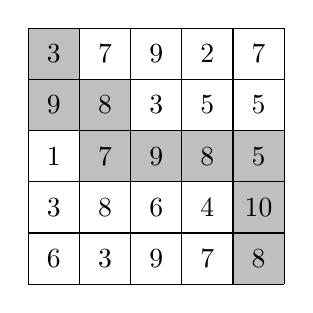
\begin{tikzpicture}[scale=.65]
  \begin{scope}
    \fill [color=lightgray] (0, 9) rectangle (1, 8);
    \fill [color=lightgray] (0, 8) rectangle (1, 7);
    \fill [color=lightgray] (1, 8) rectangle (2, 7);
    \fill [color=lightgray] (1, 7) rectangle (2, 6);
    \fill [color=lightgray] (2, 7) rectangle (3, 6);
    \fill [color=lightgray] (3, 7) rectangle (4, 6);
    \fill [color=lightgray] (4, 7) rectangle (5, 6);
    \fill [color=lightgray] (4, 6) rectangle (5, 5);
    \fill [color=lightgray] (4, 5) rectangle (5, 4);
    \draw (0, 4) grid (5, 9);
    \node at (0.5,8.5) {3};
    \node at (1.5,8.5) {7};
    \node at (2.5,8.5) {9};
    \node at (3.5,8.5) {2};
    \node at (4.5,8.5) {7};
    \node at (0.5,7.5) {9};
    \node at (1.5,7.5) {8};
    \node at (2.5,7.5) {3};
    \node at (3.5,7.5) {5};
    \node at (4.5,7.5) {5};
    \node at (0.5,6.5) {1};
    \node at (1.5,6.5) {7};
    \node at (2.5,6.5) {9};
    \node at (3.5,6.5) {8};
    \node at (4.5,6.5) {5};
    \node at (0.5,5.5) {3};
    \node at (1.5,5.5) {8};
    \node at (2.5,5.5) {6};
    \node at (3.5,5.5) {4};
    \node at (4.5,5.5) {10};
    \node at (0.5,4.5) {6};
    \node at (1.5,4.5) {3};
    \node at (2.5,4.5) {9};
    \node at (3.5,4.5) {7};
    \node at (4.5,4.5) {8};
  \end{scope}
\end{tikzpicture}
\end{center}
The sum of the numbers on the path is 67,
and this is the largest possible sum on a path
from the
upper-left corner to the lower-right corner.

We can approach the problem by
calculating for each square $(y,x)$
the maximum sum on a path
from the upper-left corner to square $(y,x)$.
Let $f(y,x)$ denote this sum,
so $f(n,n)$ is the maximum sum on a path
from the upper-left corner to
the lower-right corner.

The recursive formula is based on the observation
that a path that ends at square $(y,x)$
can come either from square $(y,x-1)$
or square $(y-1,x)$:
\begin{center}
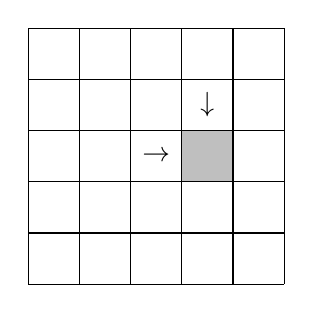
\begin{tikzpicture}[scale=.65]
  \begin{scope}
    \fill [color=lightgray] (3, 7) rectangle (4, 6);
    \draw (0, 4) grid (5, 9);
    
    \node at (2.5,6.5) {$\rightarrow$};
    \node at (3.5,7.5) {$\downarrow$};
    
  \end{scope}
\end{tikzpicture}
\end{center}

Let $r(y,x)$ denote the number in square $(y,x)$.
The base cases for the recursive function
are as follows:

\[
\begin{array}{lcl}
f(1,1) & = & r(1,1) \\
f(1,x) & = & f(1,x-1)+r(1,x) \\
f(y,1) & = & f(y-1,1)+r(y,1)\\
\end{array}
\]

In the general case there are two
possible paths, and we should select the path
that produces the larger sum:
\[ f(y,x) = \max(f(y,x-1),f(y-1,x))+r(y,x)\]

The time complexity of the solution is $O(n^2)$,
because each value $f(y,x)$ can be calculated
in constant time using the values of the
adjacent squares.

\section{Knapsack}

\index{knapsack}

\key{Knapsack} is a classic problem where we
are given $n$ objects with weights
$p_1,p_2,\ldots,p_n$ and values
$a_1,a_2,\ldots,a_n$.
Our task is to choose a subset of the objects
such that the sum of the weights is at most $x$
and the sum of the values is as large as possible.

\begin{samepage}
For example, if the objects are
\begin{center}
\begin{tabular}{rrr}
object & weight & value \\
\hline
A & 5 & 1 \\
B & 6 & 3 \\
C & 8 & 5 \\
D & 5 & 3 \\
\end{tabular}
\end{center}
\end{samepage}
and the maximum allowed total weight is 12,
an optimal solution is to select objects $B$ and $D$.
Their total weight $6+5=11$ does not exceed 12,
and their total value $3+3=6$ is the largest possible.

This task can be solved in two different ways
using dynamic programming.
We can either regard the problem as maximizing the
total value of the objects or 
minimizing the total weight of the objects.

\subsubsection{Solution 1}

\textit{Maximization:} Let $f(k,u)$
denote the largest possible total value
when a subset of objects $1 \ldots k$ is selected
such that the total weight is $u$.
The solution to the problem is
the largest value
$f(n,u)$ where $0 \le u \le x$.
A recursive formula for calculating
the function is
\[f(k,u) = \max(f(k-1,u),f(k-1,u-p_k)+a_k),\]
because we can either include or not include
object $k$ in the solution.
The base cases are $f(0,0)=0$ and $f(0,u)=-\infty$
when $u \neq 0$. The time compexity of
the solution is $O(nx)$.

In the example case, the optimal solution is
$f(4,11)=6$ that can be constructed
using the following sequence:
\[f(4,11)=f(3,6)+3=f(2,6)+3=f(1,0)+3+3=f(0,0)+3+3=6.\]

\subsubsection{Solution 2}

\textit{Minimization:} Let $f(k,u)$
denote the smallest possible total weight
when a subset of objects
$1 \ldots k$ is selected such
that the total weight is $u$.
The solution to the problem is the
largest value $u$
for which  $0 \le u \le s$ and $f(n,u) \le x$
where $s=\sum_{i=1}^n a_i$.
A recursive formula for calculating the function is
\[f(k,u) = \min(f(k-1,u),f(k-1,u-a_k)+p_k)\]
as in solution 1.
The base cases are $f(0,0)=0$ and $f(0,u)=\infty$
when $u \neq 0$.
The time complexity of the solution is $O(ns)$.

In the example case, the optimal solution is $f(4,6)=11$
that can be constructed using the following sequence:
\[f(4,6)=f(3,3)+5=f(2,3)+5=f(1,0)+6+5=f(0,0)+6+5=11.\]

~\\
It is interesting to note how the parameters of the input
affect the efficiency of the solutions.
The efficiency of solution 1 depends on the weights
of the objects, while the efficiency of solution 2
depends on the values of the objects.

\section{Edit distance}

\index{edit distance}
\index{Levenshtein distance}

The \key{edit distance} or \key{Levenshtein distance}\footnote{The distance
is named after V. I. Levenshtein who studied it in connection with binary codes \cite{lev66}.}
is the minimum number of editing operations
needed to transform a string
into another string.
The allowed editing operations are as follows:
\begin{itemize}
\item insert a character (e.g. \texttt{ABC} $\rightarrow$ \texttt{ABCA})
\item remove a character (e.g. \texttt{ABC} $\rightarrow$ \texttt{AC})
\item change a character (e.g. \texttt{ABC} $\rightarrow$ \texttt{ADC})
\end{itemize}

For example, the edit distance between
\texttt{LOVE} and \texttt{MOVIE} is 2,
because we can first perform the operation
 \texttt{LOVE} $\rightarrow$ \texttt{MOVE}
(change) and then the operation
\texttt{MOVE} $\rightarrow$ \texttt{MOVIE}
(insertion).
This is the smallest possible number of operations,
because it is clear that it is not possible
to use only one operation.

Suppose we are given strings
\texttt{x} and \texttt{y} that contain
$n$ and $m$ characters, respectively,
and we wish to calculate the edit distance
between them.
This can be done using
dynamic programming in $O(nm)$ time.
Let $f(a,b)$ denote the edit distance
between the first $a$ characters of \texttt{x}
and the first $b$ characters of \texttt{y}.
Using this function, the edit distance between
\texttt{x} and \texttt{y} equals $f(n,m)$.

The base cases for the function are
\[
\begin{array}{lcl}
f(0,b) & = & b \\
f(a,0) & = & a \\
\end{array}
\]
and in the general case the formula is
\[ f(a,b) = \min(f(a,b-1)+1,f(a-1,b)+1,f(a-1,b-1)+c),\]
where $c=0$ if the $a$th character of \texttt{x}
equals the $b$th character of \texttt{y},
and otherwise $c=1$.
The formula considers all possible ways to shorten the strings:
\begin{itemize}
\item $f(a,b-1)$ means that a character is inserted to \texttt{x}
\item $f(a-1,b)$ means that a character is removed from \texttt{x}
\item $f(a-1,b-1)$ means that \texttt{x} and \texttt{y} contain
the same character ($c=0$),
or a character in \texttt{x} is transformed into
a character in \texttt{y} ($c=1$)
\end{itemize}
The following table shows the values of $f$
in the example case:
\begin{center}
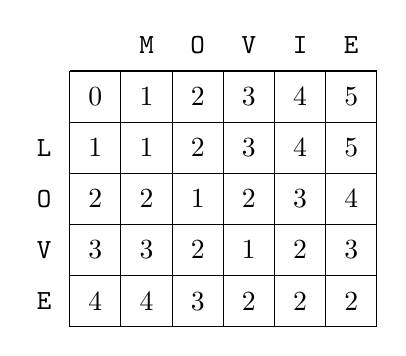
\begin{tikzpicture}[scale=.65]
  \begin{scope}
    %\fill [color=lightgray] (5, -3) rectangle (6, -4);
    \draw (1, -1) grid (7, -6);
    
    \node at (0.5,-2.5) {\texttt{L}};
    \node at (0.5,-3.5) {\texttt{O}};
    \node at (0.5,-4.5) {\texttt{V}};
    \node at (0.5,-5.5) {\texttt{E}};

    \node at (2.5,-0.5) {\texttt{M}};
    \node at (3.5,-0.5) {\texttt{O}};
    \node at (4.5,-0.5) {\texttt{V}};
    \node at (5.5,-0.5) {\texttt{I}};
    \node at (6.5,-0.5) {\texttt{E}};

    \node at (1.5,-1.5) {$0$};
    \node at (1.5,-2.5) {$1$};
    \node at (1.5,-3.5) {$2$};
    \node at (1.5,-4.5) {$3$};
    \node at (1.5,-5.5) {$4$};
    \node at (2.5,-1.5) {$1$};
    \node at (2.5,-2.5) {$1$};
    \node at (2.5,-3.5) {$2$};
    \node at (2.5,-4.5) {$3$};
    \node at (2.5,-5.5) {$4$};
    \node at (3.5,-1.5) {$2$};
    \node at (3.5,-2.5) {$2$};
    \node at (3.5,-3.5) {$1$};
    \node at (3.5,-4.5) {$2$};
    \node at (3.5,-5.5) {$3$};
    \node at (4.5,-1.5) {$3$};
    \node at (4.5,-2.5) {$3$};
    \node at (4.5,-3.5) {$2$};
    \node at (4.5,-4.5) {$1$};
    \node at (4.5,-5.5) {$2$};
    \node at (5.5,-1.5) {$4$};
    \node at (5.5,-2.5) {$4$};
    \node at (5.5,-3.5) {$3$};
    \node at (5.5,-4.5) {$2$};
    \node at (5.5,-5.5) {$2$};
    \node at (6.5,-1.5) {$5$};
    \node at (6.5,-2.5) {$5$};
    \node at (6.5,-3.5) {$4$};
    \node at (6.5,-4.5) {$3$};
    \node at (6.5,-5.5) {$2$};
  \end{scope}
\end{tikzpicture}
\end{center}

The lower-right corner of the table
tells us that the edit distance between
\texttt{LOVE} and \texttt{MOVIE} is 2.
The table also shows how to construct
the shortest sequence of editing operations.
In this case the path is as follows:

\begin{center}
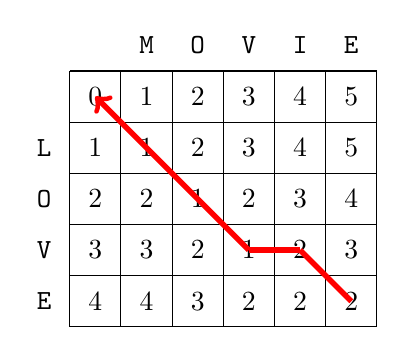
\begin{tikzpicture}[scale=.65]
  \begin{scope}
    \draw (1, -1) grid (7, -6);
    
    \node at (0.5,-2.5) {\texttt{L}};
    \node at (0.5,-3.5) {\texttt{O}};
    \node at (0.5,-4.5) {\texttt{V}};
    \node at (0.5,-5.5) {\texttt{E}};

    \node at (2.5,-0.5) {\texttt{M}};
    \node at (3.5,-0.5) {\texttt{O}};
    \node at (4.5,-0.5) {\texttt{V}};
    \node at (5.5,-0.5) {\texttt{I}};
    \node at (6.5,-0.5) {\texttt{E}};

    \node at (1.5,-1.5) {$0$};
    \node at (1.5,-2.5) {$1$};
    \node at (1.5,-3.5) {$2$};
    \node at (1.5,-4.5) {$3$};
    \node at (1.5,-5.5) {$4$};
    \node at (2.5,-1.5) {$1$};
    \node at (2.5,-2.5) {$1$};
    \node at (2.5,-3.5) {$2$};
    \node at (2.5,-4.5) {$3$};
    \node at (2.5,-5.5) {$4$};
    \node at (3.5,-1.5) {$2$};
    \node at (3.5,-2.5) {$2$};
    \node at (3.5,-3.5) {$1$};
    \node at (3.5,-4.5) {$2$};
    \node at (3.5,-5.5) {$3$};
    \node at (4.5,-1.5) {$3$};
    \node at (4.5,-2.5) {$3$};
    \node at (4.5,-3.5) {$2$};
    \node at (4.5,-4.5) {$1$};
    \node at (4.5,-5.5) {$2$};
    \node at (5.5,-1.5) {$4$};
    \node at (5.5,-2.5) {$4$};
    \node at (5.5,-3.5) {$3$};
    \node at (5.5,-4.5) {$2$};
    \node at (5.5,-5.5) {$2$};
    \node at (6.5,-1.5) {$5$};
    \node at (6.5,-2.5) {$5$};
    \node at (6.5,-3.5) {$4$};
    \node at (6.5,-4.5) {$3$};
    \node at (6.5,-5.5) {$2$};

    \path[draw=red,thick,-,line width=2pt] (6.5,-5.5) -- (5.5,-4.5);
    \path[draw=red,thick,-,line width=2pt] (5.5,-4.5) -- (4.5,-4.5);
    \path[draw=red,thick,->,line width=2pt] (4.5,-4.5) -- (1.5,-1.5);
  \end{scope}
\end{tikzpicture}
\end{center}

The last characters of \texttt{LOVE} and \texttt{MOVIE}
are equal, so the edit distance between them
equals the edit distance between \texttt{LOV} and \texttt{MOVI}.
We can use one editing operation to remove the
character \texttt{I} from \texttt{MOVI}.
Thus, the edit distance is one larger than
the edit distance between \texttt{LOV} and \texttt{MOV}, etc.

\section{Counting tilings}

Sometimes the states of a dynamic programming solution
are more complex than fixed combinations of numbers.
As an example,
we consider the problem of calculating
the number of distinct ways to
fill an $n \times m$ grid using
$1 \times 2$ and $2 \times 1$ size tiles.
For example, one valid solution
for the $4 \times 7$ grid is
\begin{center}
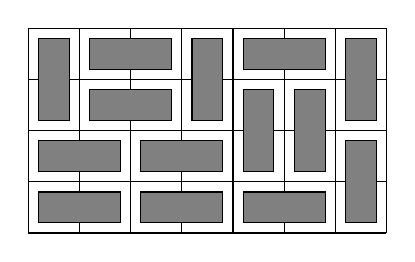
\begin{tikzpicture}[scale=.65]
    \draw (0,0) grid (7,4);
    \draw[fill=gray] (0+0.2,0+0.2) rectangle (2-0.2,1-0.2);
    \draw[fill=gray] (2+0.2,0+0.2) rectangle (4-0.2,1-0.2);
    \draw[fill=gray] (4+0.2,0+0.2) rectangle (6-0.2,1-0.2);
    \draw[fill=gray] (0+0.2,1+0.2) rectangle (2-0.2,2-0.2);
    \draw[fill=gray] (2+0.2,1+0.2) rectangle (4-0.2,2-0.2);
    \draw[fill=gray] (1+0.2,2+0.2) rectangle (3-0.2,3-0.2);
    \draw[fill=gray] (1+0.2,3+0.2) rectangle (3-0.2,4-0.2);
    \draw[fill=gray] (4+0.2,3+0.2) rectangle (6-0.2,4-0.2);

    \draw[fill=gray] (0+0.2,2+0.2) rectangle (1-0.2,4-0.2);
    \draw[fill=gray] (3+0.2,2+0.2) rectangle (4-0.2,4-0.2);
    \draw[fill=gray] (6+0.2,2+0.2) rectangle (7-0.2,4-0.2);
    \draw[fill=gray] (4+0.2,1+0.2) rectangle (5-0.2,3-0.2);
    \draw[fill=gray] (5+0.2,1+0.2) rectangle (6-0.2,3-0.2);
    \draw[fill=gray] (6+0.2,0+0.2) rectangle (7-0.2,2-0.2);

\end{tikzpicture}
\end{center}
and the total number of solutions is 781.

The problem can be solved using dynamic programming
by going through the grid row by row.
Each row in a solution can be represented as a
string that contains $m$ characters from the set
$\{\sqcap, \sqcup, \sqsubset, \sqsupset \}$.
For example, the above solution consists of four rows
that correspond to the following strings:
\begin{itemize}
\item
$\sqcap \sqsubset \sqsupset \sqcap \sqsubset \sqsupset \sqcap$
\item
$\sqcup \sqsubset \sqsupset \sqcup \sqcap \sqcap \sqcup$
\item
$\sqsubset \sqsupset \sqsubset \sqsupset \sqcup \sqcup \sqcap$ 
\item
$\sqsubset \sqsupset \sqsubset \sqsupset \sqsubset \sqsupset \sqcup$
\end{itemize}

Let $f(k,x)$ denote the number of ways to
construct a solution for rows $1 \ldots k$
in the grid so that string $x$ corresponds to row $k$.
It is possible to use dynamic programming here,
because the state of a row is constrained
only by the state of the previous row.

A solution is valid if row $1$ does not contain
the character $\sqcup$,
row $n$ does not contain the character $\sqcap$,
and all consecutive rows are \emph{compatible}.
For example, the rows
$\sqcup \sqsubset \sqsupset \sqcup \sqcap \sqcap \sqcup$ and
$\sqsubset \sqsupset \sqsubset \sqsupset \sqcup \sqcup \sqcap$ 
are compatible, while the rows
$\sqcap \sqsubset \sqsupset \sqcap \sqsubset \sqsupset \sqcap$ and
$\sqsubset \sqsupset \sqsubset \sqsupset \sqsubset \sqsupset \sqcup$
are not compatible.

Since a row consists of $m$ characters and there are
four choices for each character, the number of distinct
rows is at most $4^m$.
Thus, the time complexity of the solution is
$O(n 4^{2m})$ because we can go through the
$O(4^m)$ possible states for each row,
and for each state, there are $O(4^m)$
possible states for the previous row.
In practice, it is a good idea to rotate the grid
so that the shorter side has length $m$,
because the factor $4^{2m}$ dominates the time complexity.

It is possible to make the solution more efficient
by using a more compact representation for the rows.
It turns out that it is sufficient to know which
columns of the previous row contain the upper square
of a vertical tile.
Thus, we can represent a row using only characters
$\sqcap$ and $\Box$, where $\Box$ is a combination
of characters
$\sqcup$, $\sqsubset$ and $\sqsupset$.
Using this representation, there are only
$2^m$ distinct rows and the time complexity is
$O(n 2^{2m})$.

As a final note, there is also a surprising direct formula
for calculating the number of tilings:
% \footnote{Surprisingly,
% this formula was discovered independently
% by \cite{kas61} and \cite{tem61} in 1961.}:
\[ \prod_{a=1}^{\lceil n/2 \rceil} \prod_{b=1}^{\lceil m/2 \rceil} 4 \cdot (\cos^2 \frac{\pi a}{n + 1} + \cos^2 \frac{\pi b}{m+1})\]
This formula is very efficient, because it calculates
the number of tilings in $O(nm)$ time,
but since the answer is a product of real numbers,
a practical problem in using the formula is
how to store the intermediate results accurately.


